\documentclass[11pt,a4paper]{article}

\usepackage[utf8]{inputenc}
\usepackage[T1]{fontenc}
\usepackage{geometry}
\geometry{margin=2cm, top=2.5cm, bottom=2.5cm}
\usepackage{times}
\usepackage{booktabs}
\usepackage{enumitem}
\usepackage{tikz}
\usetikzlibrary{arrows.meta, positioning, shapes.geometric, calc}
\usepackage{caption}
\usepackage{float}
\usepackage{titlesec}
\usepackage{fancyhdr}
\usepackage{multicol}

% ===== TIKZ STYLES (BLACK AND WHITE, CLEAN) =====
\tikzset{
  box/.style={draw=black, rectangle, align=center, inner sep=2mm, minimum height=0.8cm, font=\small, thick, fill=white},
  widebox/.style={box, minimum width=10cm},
  arrow/.style={-Latex, thick, draw=black},
  dasharrow/.style={-Latex, thick, dashed, draw=black}
}

\pagestyle{fancy}
\fancyhf{}
\fancyhead[C]{\small\textit{ProfsAgent --- System Pipeline and Evaluation Framework}}
\fancyfoot[C]{\thepage}
\renewcommand{\headrulewidth}{0.4pt}

\titlespacing*{\section}{0pt}{10pt}{5pt}
\titlespacing*{\subsection}{0pt}{8pt}{4pt}
\setlength{\parskip}{4pt}
\setlength{\parindent}{0pt}

\title{
\vspace{-1cm}
\textbf{ProfsAgent: An Agentic AI System for\\End-to-End Course Design and Delivery Planning}\\[0.3cm]
\large System Pipeline, Stage Specifications, and Evaluation Framework
}
\author{Vihan Ahlawat \quad Parth Malik \quad Amit Kumar\\[0.1cm]
\small Supervisors: Prof.\ Pankaj Jalote \quad Prof.\ Jainendra Shukla\\
\small Indraprastha Institute of Information Technology, Delhi}
\date{September 2026}

\begin{document}
\maketitle
\thispagestyle{fancy}

% ======================================================================
\section{Introduction}
% ======================================================================

Designing a high-quality course requires defining objectives, structuring topics, preparing materials, and creating assessments---all of which must remain pedagogically aligned. In practice, these components are often designed independently, leading to inconsistencies such as learning outcomes that are never assessed, or workloads exceeding available teaching time.

\textbf{ProfsAgent} is an AI assistant that treats course design as a \textit{connected system}. The core philosophy is:
\begin{center}
\textbf{Context Input $\to$ AI Generation $\to$ Automated Validation $\to$ Professor Review $\to$ Refinement}
\end{center}

% ======================================================================
\section{System Pipeline Overview}
% ======================================================================

Figure~\ref{fig:pipeline} shows the simplified high-level workflow, moving from institutional context collection to the final course package.

\begin{figure}[H]
\centering
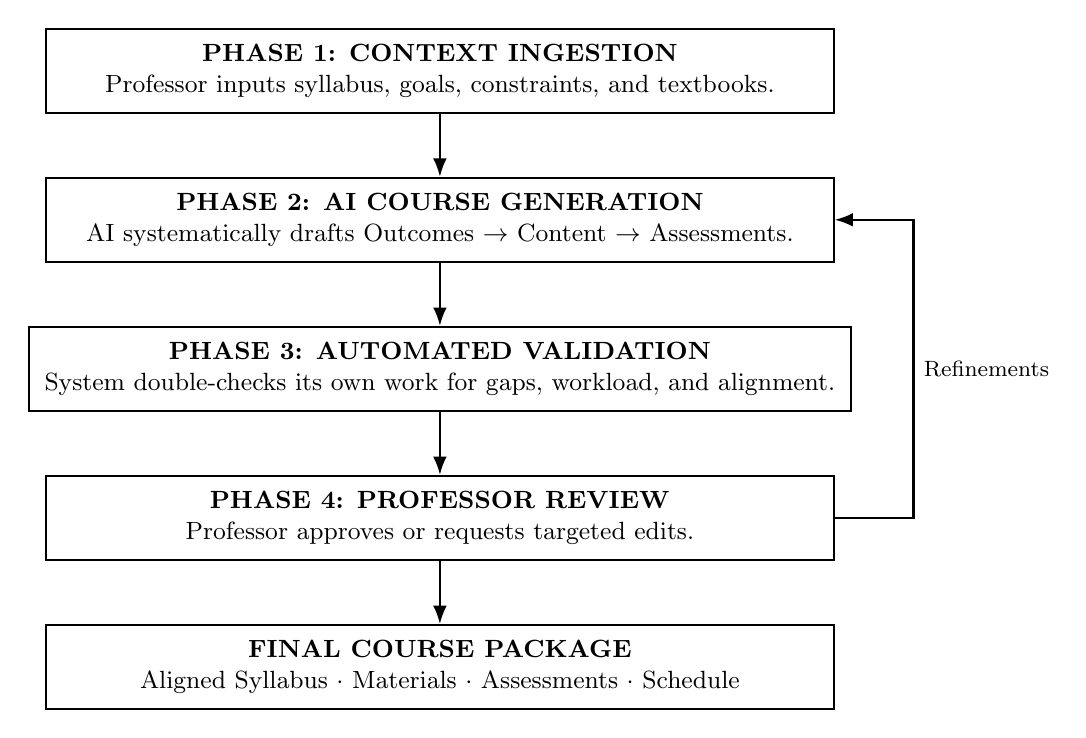
\begin{tikzpicture}[node distance=0.8cm]

\node[widebox] (p1) {\textbf{PHASE 1: CONTEXT INGESTION}\\Professor inputs syllabus, goals, constraints, and textbooks.};
\node[widebox, below=of p1] (p2) {\textbf{PHASE 2: AI COURSE GENERATION}\\AI systematically drafts Outcomes $\to$ Content $\to$ Assessments.};
\node[widebox, below=of p2] (p3) {\textbf{PHASE 3: AUTOMATED VALIDATION}\\System double-checks its own work for gaps, workload, and alignment.};
\node[widebox, below=of p3] (p4) {\textbf{PHASE 4: PROFESSOR REVIEW}\\Professor approves or requests targeted edits.};
\node[widebox, below=of p4] (p5) {\textbf{FINAL COURSE PACKAGE}\\Aligned Syllabus $\cdot$ Materials $\cdot$ Assessments $\cdot$ Schedule};

\draw[arrow] (p1) -- (p2);
\draw[arrow] (p2) -- (p3);
\draw[arrow] (p3) -- (p4);
\draw[arrow] (p4) -- (p5);
\draw[arrow] (p4.east) -- ++(1,0) |- node[right, near start] {\footnotesize Refinements} (p2.east);

\end{tikzpicture}
\caption{Simplified ProfsAgent Workflow}
\label{fig:pipeline}
\end{figure}

\clearpage

% ======================================================================
\section{Pipeline Phases: Inputs, Processing, and Outputs}
% ======================================================================

% ---------- PHASE 1 ----------
\subsection*{Phase 1: Context Ingestion (The "Input" Phase)}
\textbf{What it does:} The system reads the professor's constraints, existing syllabi, program goals, and reference textbooks to build a "course brain". This grounds the AI so it generates content specific to the institution, preventing generic hallucinations.

\textbf{Input:} Course title, credit structure, semester length, reference materials, and teaching preferences.

\textbf{Output:} A structured set of rules and a searchable knowledge base specific to the course.

% ---------- PHASE 2 ----------
\subsection*{Phase 2: AI Course Generation (The "Module Generation" Phase)}
\textbf{What it does:} Instead of generating a course in one massive text dump, ProfsAgent breaks the problem down into three sequential steps, ensuring pedagogical alignment from start to finish.

\begin{figure}[H]
\centering
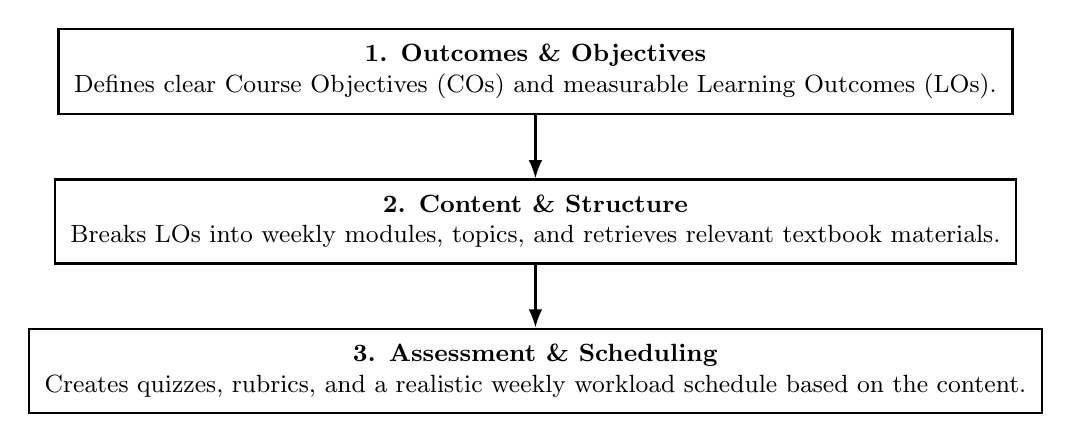
\begin{tikzpicture}[node distance=0.8cm]

\node[box, minimum width=12cm] (step1) {\textbf{1. Outcomes \& Objectives}\\Defines clear Course Objectives (COs) and measurable Learning Outcomes (LOs).};

\node[box, below=of step1, minimum width=12cm] (step2) {\textbf{2. Content \& Structure}\\Breaks LOs into weekly modules, topics, and retrieves relevant textbook materials.};

\node[box, below=of step2, minimum width=12cm] (step3) {\textbf{3. Assessment \& Scheduling}\\Creates quizzes, rubrics, and a realistic weekly workload schedule based on the content.};

\draw[arrow] (step1) -- (step2);
\draw[arrow] (step2) -- (step3);

\end{tikzpicture}
\caption{Linear Course Generation Flow}
\label{fig:generation}
\end{figure}

\textbf{Input:} The "course brain" from Phase 1.

\textbf{Output:} A fully drafted set of Course Outcomes, Weekly Modules, Lecture Topics, Recommended Readings, and Assessments.

\clearpage

% ---------- PHASE 3 ----------
\subsection*{Phase 3: Automated Validation (The "Quality Check" Phase)}

\textbf{What it does:} Before showing anything to the professor, the system double-checks its own work using strict rules (not just AI guessing). It ensures the course is actually teachable and consistent.

\begin{figure}[H]
\centering
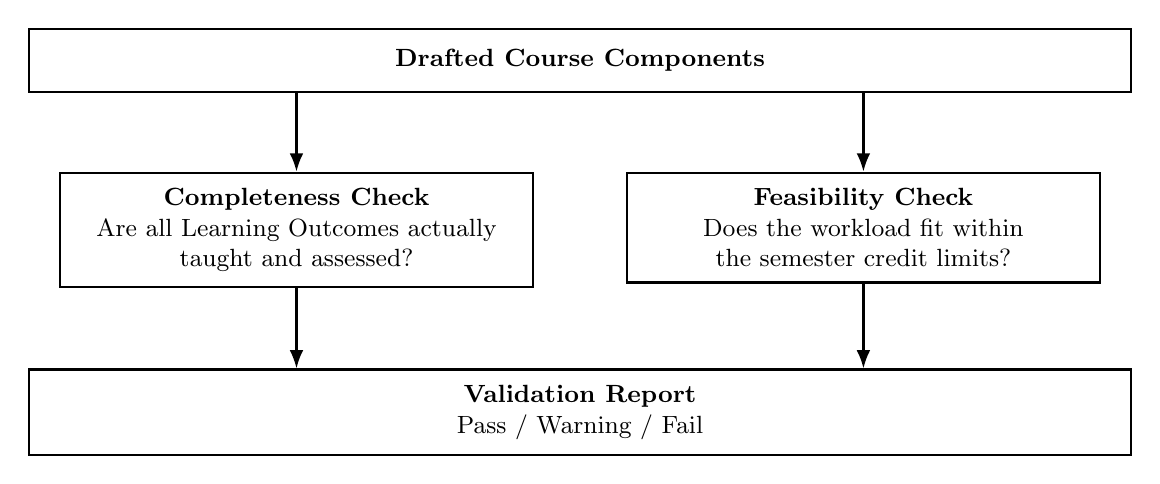
\begin{tikzpicture}[node distance=0.8cm and 0.5cm]

\node[widebox, minimum width=14cm] (input) {\textbf{Drafted Course Components}};

\node[box, below=1cm of input, xshift=-3.6cm, minimum width=6cm] (g1) {\textbf{Completeness Check}\\Are all Learning Outcomes actually\\taught and assessed?};

\node[box, below=1cm of input, xshift=3.6cm, minimum width=6cm] (c1) {\textbf{Feasibility Check}\\Does the workload fit within\\the semester credit limits?};

\node[widebox, below=3.5cm of input, minimum width=14cm] (rep) {\textbf{Validation Report}\\Pass / Warning / Fail};

\draw[arrow] (input.south -| g1.north) -- (g1.north);
\draw[arrow] (input.south -| c1.north) -- (c1.north);
\draw[arrow] (g1.south) -- (g1.south |- rep.north);
\draw[arrow] (c1.south) -- (c1.south |- rep.north);

\end{tikzpicture}
\caption{Automated Validation Checks}
\label{fig:validation}
\end{figure}

\textbf{Input:} The drafted course from Phase 2.

\textbf{Output:} A validation report highlighting any broken links (e.g., "Week 3 has an assessment on a topic that hasn't been taught yet").

% ---------- PHASE 4 ----------
\subsection*{Phase 4: Professor Review \& Feedback Loop (Human-in-the-Loop)}

\begin{figure}[H]
\centering
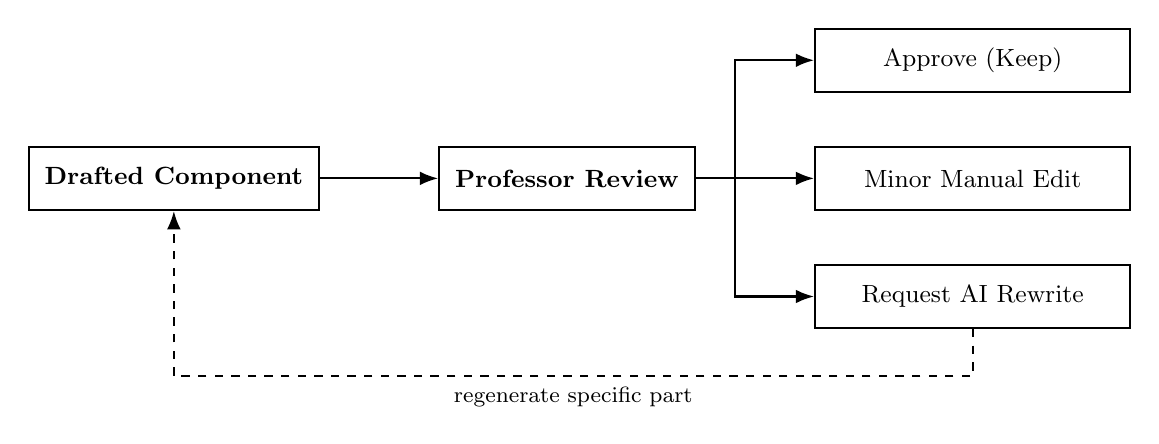
\begin{tikzpicture}[node distance=1.5cm]

\node[box, minimum width=3cm] (gen) {\textbf{Drafted Component}};
\node[box, right=of gen, minimum width=3cm] (rev) {\textbf{Professor Review}};

\node[box, right=of rev, yshift=1.5cm, minimum width=4cm] (o1) {Approve (Keep)};
\node[box, right=of rev, yshift=0cm, minimum width=4cm] (o2) {Minor Manual Edit};
\node[box, right=of rev, yshift=-1.5cm, minimum width=4cm] (o3) {Request AI Rewrite};

\draw[arrow] (gen) -- (rev);
\draw[arrow] (rev.east) -- ++(0.5,0) |- (o1.west);
\draw[arrow] (rev.east) -- ++(0.5,0) |- (o2.west);
\draw[arrow] (rev.east) -- ++(0.5,0) |- (o3.west);

\draw[dasharrow] (o3.south) -- ++(0,-0.6) -| node[below, near start]{\footnotesize regenerate specific part} (gen.south);

\end{tikzpicture}
\caption{Professor Feedback Loop}
\label{fig:feedback}
\end{figure}

\textbf{What it does:} The professor is the final decision-maker. They can review and approve individual pieces. If they ask the AI to rewrite a topic, the system smartly ripples that change through related assessments without having to regenerate the entire course from scratch.

\textbf{Output:} The finalized, classroom-ready Course Package.

\clearpage

% ======================================================================
\section{Research Evaluation Framework}
% ======================================================================

\begin{figure}[H]
\centering
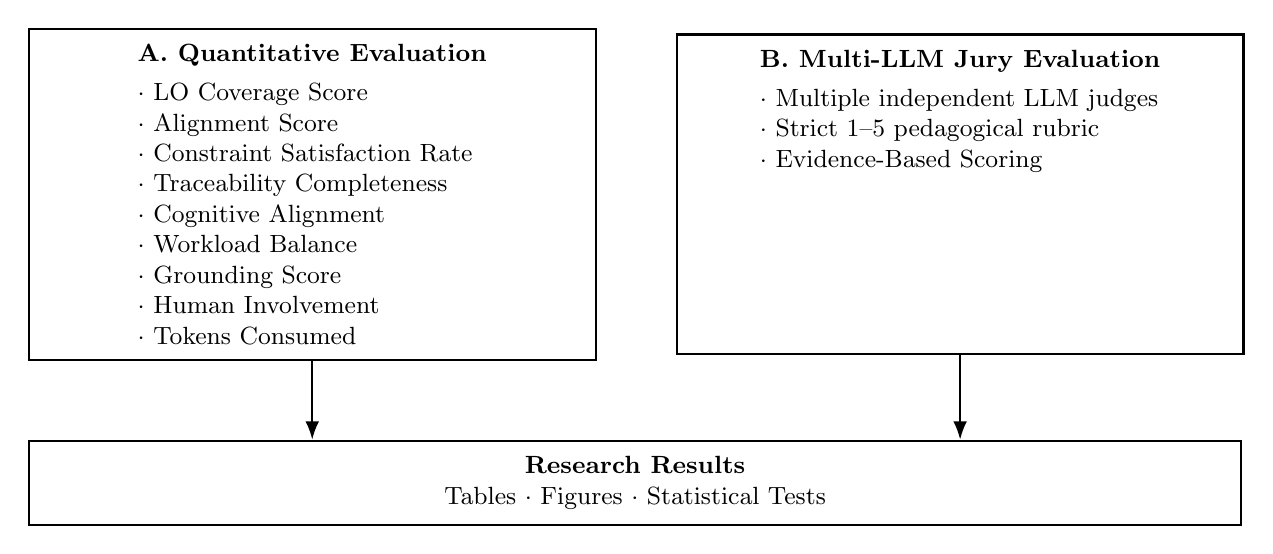
\begin{tikzpicture}[node distance=0.8cm and 1cm]

\node[box, minimum width=7.2cm, align=left] (q1) {\textbf{A. Quantitative Evaluation}\\[3pt]
$\cdot$ LO Coverage Score\\
$\cdot$ Alignment Score\\
$\cdot$ Constraint Satisfaction Rate\\
$\cdot$ Traceability Completeness\\
$\cdot$ Cognitive Alignment\\
$\cdot$ Workload Balance\\
$\cdot$ Grounding Score\\
$\cdot$ Human Involvement\\
$\cdot$ Tokens Consumed};

\node[box, right=of q1, minimum width=7.2cm, align=left] (q2) {\textbf{B. Multi-LLM Jury Evaluation}\\[3pt]
$\cdot$ Multiple independent LLM judges\\
$\cdot$ Strict 1--5 pedagogical rubric\\
$\cdot$ Evidence-Based Scoring\\[5.5em]};

\node[widebox, below=1cm of q1, xshift=4.1cm, minimum width=15.4cm] (res) {\textbf{Research Results}\\Tables $\cdot$ Figures $\cdot$ Statistical Tests};

\draw[arrow] (q1.south) -- (q1.south |- res.north);
\draw[arrow] (q2.south) -- (q2.south |- res.north);

\end{tikzpicture}
\caption{Research Evaluation Framework}
\label{fig:eval}
\end{figure}

\subsection*{A. Quantitative Evaluation (Automated Metrics)}
\begin{itemize}[nosep,leftmargin=1.5em]
\item \textbf{LO Coverage Score:} Percentage of LOs that are taught and assessed.
\item \textbf{Alignment Score:} Semantic similarity and graph linkage between CO$\leftrightarrow$LO$\leftrightarrow$Topic$\leftrightarrow$Assessment.
\item \textbf{Constraint Satisfaction Rate:} Percentage of institutional constraints met.
\item \textbf{Traceability Completeness:} Ratio of components with valid Knowledge Graph linkages.
\item \textbf{Cognitive Alignment Score:} Match between Assessment Bloom's level and LO Bloom's level.
\item \textbf{Human Involvement:} Total number of human interventions and time spent editing.
\item \textbf{Tokens Consumed:} Total prompt and completion tokens used for cost analysis.
\end{itemize}

\subsection*{B. Multi-LLM Rubric-Based Course Quality Evaluation}
Instead of relying solely on expensive human panels, the system employs a multi-LLM jury evaluation to measure pedagogical quality and coherence.
\begin{itemize}[nosep,leftmargin=1.5em]
\item \textbf{Independent Jury:} Multiple LLMs (e.g., GPT-4, Claude, Gemini) act as independent judges.
\item \textbf{Multi-Dimensional Rubric (1--5 Scale):} Judges score specific dimensions including LO Quality, Course Structure, Constructive Alignment, Teaching Material, Assessment, and Usability.
\item \textbf{Evidence-Based Scoring:} LLMs must justify their scores using explicit evidence from the course knowledge graph and generated artifacts.
\end{itemize}

\end{document}
